


\documentclass[tikz,border=2mm]{standalone}
\usepackage{tikz}
\usetikzlibrary{arrows}
\usetikzlibrary{arrows.meta,automata,positioning}

\begin{document}

% \usetikzlibrary{arrows.meta,automata,positioning}
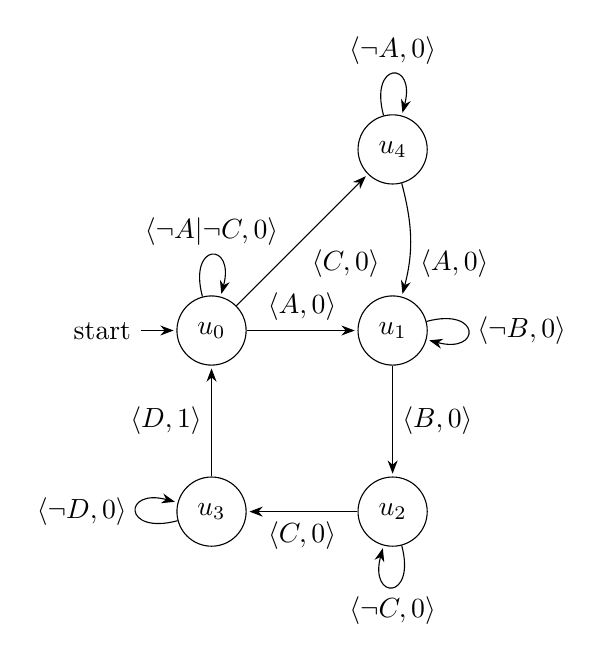
\begin{tikzpicture}[>=Stealth, shorten >=1pt, node distance=2.3cm, on grid, auto]

% Nodes
\node[state, initial] (u0) {$u_0$};
\node[state] (u1) [right=of u0] {$u_1$};
\node[state] (u2) [below=of u1] {$u_2$};
\node[state] (u3) [left=of u2] {$u_3$};
\node[state] (u4) [above=of u1] {$u_4$}; % New node u4

% Edges with labels
\path[->]
    (u0) edge[loop above] node {$\langle \neg A|\neg C, 0 \rangle$} ()
         edge node {$\langle A, 0 \rangle$} (u1)
         edge  node[below right] {$\langle C, 0 \rangle$} (u4) % Edge to u4
        (u4) edge[loop above] node {$\langle \neg A , 0 \rangle$} ()
    (u4) edge[bend left=15] node[below right] {$\langle A, 0 \rangle$} (u1) % Edge from u4 to u1
    (u1) edge[loop right] node {$\langle \neg B, 0 \rangle$} ()
         edge node {$\langle B, 0 \rangle$} (u2)
    (u2) edge[loop below] node {$\langle \neg C, 0 \rangle$} ()
         edge node {$\langle C, 0 \rangle$} (u3)
    (u3) edge[loop left] node {$\langle \neg D, 0 \rangle$} ()
         edge node {$\langle D, 1 \rangle$} (u0);

\end{tikzpicture}


\end{document}